\def\year{2015}
%File: formatting-instruction.tex
\documentclass[letterpaper]{article}
\usepackage{aaai}
\usepackage{times}
\usepackage{helvet}
\usepackage{courier}
\usepackage{color}
\frenchspacing
\setlength{\pdfpagewidth}{8.5in}
\setlength{\pdfpageheight}{11in}
\pdfinfo{
/Title (Insert Your Title Here)
/Author (Put All Your Authors Here, Separated by Commas)}
\setcounter{secnumdepth}{0}
\usepackage{amsmath}  
\usepackage{amsfonts}
\DeclareMathOperator*{\argmin}{\arg\!\min} 
\DeclareMathOperator*{\argmax}{\arg\!\max} 
\usepackage{graphicx}

\newif\ifnotes

%---------Toggle these flags if you want to supress the comments------------
\notestrue
%\notesfalse
%-----------------------------------------------------------------------------

\ifnotes
\newcommand{\sw}[1]{\textcolor{red}{SW: #1}}
\newcommand{\jm}[1]{\textcolor{blue}{Joao: #1}}
\else
\newcommand{\sw}[1]{}
\newcommand{\jm}[1]{}
\fi

 \begin{document}
% The file aaai.sty is the style file for AAAI Press 
% proceedings, working notes, and technical reports.
%
\title{Inverse Reinforcement Learning from Failure}
% \author{AAAI Press\\
% Association for the Advancement of Artificial Intelligence\\
% 2275 East Bayshore Road, Suite 160\\
% Palo Alto, California 94303\\
% }
\maketitle
\begin{abstract}
\begin{quote}
In this paper, we approach the problem of Inverse Reinforcement Learning (IRL) from a rather different perspective. Instead of trying to only mimic an expert as in traditional IRL, we present a method that is capable of learning from data we would like to avoid \sw{what does it mean to avoid data? you mean avoid the behavior that caused the data? also, this sounds like we are *only* learning from bad data}. In particular, we propose a new IRL algorithm that extends the state-of-the-art method of Maximum Entropy Inverse Reinforcement Learning to exploit such failed demonstrations \sw{this sounds very incremental; focus on the conceptual leap we propose rather than on what it extends}. Our experimental results \sw{say something about the domains emphasising the real-world aspects} show that learning in this fashion allows for better generalisation \sw{what about better performance? wrt both expert and taboo reward functions}, especially in the presence of limited data. \sw{which data is limited? good, bad, or both?}
\end{quote}
\end{abstract}

\section{Introduction}
	Inverse Reinforcement Learning (IRL) \cite{ng2000algorithms}, along with the closely related field of Inverse Optimal Control (IOC) allow a machines to learn cost functions for various decision making tasks, from human demonstration.  This is especially fit for tasks that can be easily demonstrated whilst the cost function is hard to formalise, a classic example being car driving. In addition because the output of the algorithm is a cost function, instead of a direct mapping to actions (a policy), it is more robust to changes in the environment and therefore more transferable to novel domains.\\
	All Inverse Reinforcement Learning methods to date focus on imitation of a certain type of behaviour. There are however, tasks for which we might have data that demonstrate behaviour that we would like to avoid. Consider for example tasks which are learned using trial and error where demonstrations of both successful and failed behaviour are available, and labeling them as such is straightforward. This plentiful data source could be extremely halpful for learning and unfortunately current methods provide no means of leveraging it. Furthermore, only having access to behaviours we would like to immitate could leave ambiguity at certain important situations that are never encountered in the data. It could also be the case that for some tasks, demonstrating the behaviour to be avoided is in fact easier than demonstrating successful behaviour, which could require great expertise. For example if we want a robot not to hit obstacles, we would simulate the robot actually crashing, and then use that data to learn to avoid the undesired behaviour in the real world. Finally, learning to avoid behaviours could be usefull in Active and Lifelong Learning since a human would be able to specify behaviours of the agent that are undesirable at the trajectory level (instead of the action level). 

	 Starting from Maximum Causal Entropy IRL \cite{ziebart2010modelingthesis} we first present the mathematical modifications that allow the incorporation of failed demonstrations into the learning process. We then present the IRL-F algorithm, the first IRL algorithm that can learn useful reward functions from both behaviour that we want to match (successful) and behaviour that we want to avoid (failed). We go on to apply the algorithm to synthetic and real world data. On synnthetic data the results demonstrate the algorithm's ability to generalise better in the presense of limited training data with little extra computational cost. We further demonstrate the algorithm's ability to learn mixtures of behaviours, which is highly desirable in the presence of sub-optimal experts. Finally, on real robotic navigation data the algorithm yields consistently superior results when compared to the state-of-the art \sw{vague: give specifics about performance}. 

\section{Background}
Most IRL methods are grounded on a formalization of the underlying decision-making problem as a Markov Decision Process (MDP). An MDP represents a discrete-time decision making process wherein the actions of an agent may have a stochastic influence on its environment. In an MDP, at step $t$, the system (which includes the agent and its environment) is known to be in a \emph{state} $s_t\in\mathbf{S}$; the agent selects an action $a_t\in\mathbf{A}$; the agent is then awarded a real-valued \emph{reward} for performing that action, and the system jumps to state $s_{t+1}$ with probability $P(s'|s,a)$. An MDP is formally defined as a tuple $\langle\mathbf{S},\mathbf{A},\mathcal{T},R\rangle$, where $\mathbf{S}$ and $\mathbf{A}$ are sets of discrete states and actions respectively, $\mathcal{T}:\mathbf{S}\times\mathbf{A}\times\mathbf{S}\rightarrow [0,1]$ is a transition function such that $\mathcal T(s,a,s')=P(s'|s,a)$, and $R:\mathbf{S}\times\mathbf{A}\rightarrow\mathbb R$ is the reward function. 
Optimally solving an MDP involves finding a policy $\pi:\mathbf{A}\times\mathbf{S}\rightarrow[0,1]$ with $\pi(a,s) = P(a\,|\,s)$, which maximises the expected (discounted) sum of rewards over a fixed number $h$ of decisions. This expectation can be expressed as the \emph{value} of policy $\pi$:
\begin{equation}
\label{eq:value}
 V^\pi(s) = E\{\sum_{t = 1}^h \gamma^{t-1}R(s_t,a_t)\,\vert\, s_1 = s\} \quad,
\end{equation}
where $\gamma\in]0,1]$ is a discount factor, that expresses the degree of preference for immediate rewards.

IRL methods focus on scenarios where the reward function $R$ is initially unknown, and must be learned from examples of the behavior of an agent. In that context, we are provided with an `incomplete' MDP $\langle\mathbf{S},\mathbf{A},\mathcal{T}\rangle$, also known as an MDP/R. Although the reward function is unknown, it is typical to assume that it can be parametrized in terms of $K$ \emph{feature functions}, $\phi_k(s,a)$:
\begin{equation}
R(s,a) = \sum_{k=1}^Kw_k\phi_k(s,a)\quad, \label{eq:rew}
\end{equation}
where $w_k$ are the weights for each feature. The feature functions are also assumed to be known to the learner. Using this representation, the goal of IRL is to learn the weight vector $w=[w_1\,w_2\,\ldots\,w_k]^T$.

From \eqref{eq:value} and \eqref{eq:rew}, a parametric form of the value function can also be obtained, by noting that the weights $w_k$ are time-invariant:

\begin{align}
 	V^{\pi}(s) &= \sum^K_{k=1}w_k\left(E\{\sum_{t = 1}^h \gamma^{t-1}\phi_k(s_t,a_t)\,\vert\, s_1 = s\}\right)\\
&= \sum^K_{k=1}w_k\mu^\pi_k\quad,
\end{align}
where $\mu^{\pi}_k$ represents the bracketed term, and is known as the $k-$th \emph{feature expectation}, which describes the (discounted) accumulation of feature $\phi_k$ by the agent over time, while following policy $\pi$.

In addition to this parametrisation, the algorithm is provided with a dataset ${\mathcal{D}}$ of $N$ trajectories $\tau$, each of possibly varying length $l({\tau})$ \jm{$|\tau_n|$ could also work} and consisting of state-action sequences from $\mathbf{S}$ and $\mathbf{A}$ respectively. The dataset can therefore be summarised as $\mathcal{D}:\big\{ \tau_1,\tau_2,...\tau_N \big\}$ where $\tau_n = \{(s_1,a_1),(s_2,a_2),...(s_{l({\tau_n})},a_{l({\tau_n})})\}$.

From the dataset ${\mathcal{D}}$ we can derive a similar quantity known as the empirical feature expectation:

\begin{equation}
	\widetilde{\mu}^{\mathcal{D}}_k =\frac{1}{N}\sum_{\tau\in\mathcal{D}}\sum_{t=1}^{l({\tau})}\phi_k(s^\tau_t,a^\tau_t)\quad. \label{eqn:empirical_fe}
\end{equation}

The aim of an inverse reinforcement learning algorithm is to find the configuration of weights $w$ that brings the vectors $\widetilde\mu^{\mathcal{D}}~=~[\widetilde\mu^{\mathcal{D}}_1\,\ldots\,\widetilde\mu^{\mathcal{D}}_k]^T$ and $\mu^{\pi}~=~[\mu^\pi_1\,\ldots\,\mu^\pi_k]$ together according to some metric, while maintaining the capability to generalise to unseen initial conditions.

Different algorithms cast the IRL problem to existing, mature and reliable frameworks such as structured prediction \cite{ratliff2006maximum} and Bayesian inference \cite{ramachandran2007bayesian}, while others rely on non-linear representation of the reward such as Gaussian processes \cite{levine2011nonlinear}, Neural Networks, and Decision Trees \cite{ratliff200w7boosting}. 

Despite theoretical differences, most IRL algorithms share a learning pipeline that proceeds as follows. An initial guess for the cost/reward function is input to a planner which produces a policy or a control law. Using this policy we can then simulate a decision making task from the same initial conditions as our dataset. After comparing the model's behaviour ($\mu^{\pi}$)  with the data ($\widetilde{\mu}^{\mathcal{D}}$), a cost function update is performed to bring the two quantities closer together.

In this paper we concentrate on two similar methods introduced by Ziebart in \cite{ziebart2008maximum} and \cite{ziebart2010modelingthesis}, and cast the problem in terms of finding the maximum entropy policy that explains the state-action trajectories contained in the dataset. Maximum-entropy methods are particularly atractive because of their probabilistic formulation, which makes them robust to noise and sub-optimal experts\jm{needs to be re-worded}, and results in convex optimisation problems. The methods are rooted in the following optimisation.\jm{$\mu_{s_0,k}$ undefined}

\begin{align}
	\hbox{find:}\quad &\max\limits_{\pi(a,s)} H(\mathbf{A}^h||\mathbf{S}^h)\\
\hbox{subject to:}\quad &\widetilde{\mu}^{\mathcal{D}}_k   = \mu^{\pi}_{s_0,k} \quad \forall k \label{eq:good_ineq}\\
\hbox{and:}\quad &\sum_{a\in\mathbf{A}}\pi(a,s)  = 1 \quad \forall s\in\mathbf{S}\\
\hbox{and:}\quad &\pi(a,s)  > 0 \quad \forall s\in\mathbf{S},a\in\mathbf{A}  
\end{align}

Where $H(\mathbf{A}^h||\mathbf{S}^h)$ is the conditional entropy of all possible action sequences of length $h$, causally conditioned on all possible state sequences, also of length $h$. For MDPs this quantity is fully determined given a policy $\pi$ and a transition function $\mathcal{T}$:
\begin{align}
H(\mathbf{A}^T||\mathbf{S}^T) = \sum_{t=1}^T \sum_{s_t,a_t} P(a_t,s_t)\log(P(a_t|s_t))\quad,
\label{eg:entdef}
\end{align}
where:
\begin{align*}
  P(a_t,s_t)&= P(a_t|s_t)P(s_t|s_{t-1},a_{t-1})P(s_{t-1},a_{t-1})\\
  &=\pi(a_t,s_t)\mathcal T(s_{t-1},a_{t-1},s_t)P(s_{t-1},a_{t-1})\quad.
\end{align*}
	
 The policy is further constrained to match the feature expectations, defined in Equations \eqref{eqn:model_fe} and \eqref{eqn:empirical_fe}. The optimisation problem is solved using the method of Lagrange multipliers, which elegantly intoduces the notion of a reward function in to the resulting Lagrangian. The solution proceeds with a planning step aimed at maximising this Lagrangian with respect to the policy. Planning in this framework takes place as a version of the Bellman equation \cite{sutton1998reinforcement} where the max operator is replaced with a softmax.

	\begin{equation}
		\begin{split}
	&Q_w(s,a)^{soft} = R(s,a) + \sum_{s'}T(s,a,s')V_w(s')\\	
	&V_w(s)^{soft} = \log\sum_{a}exp(Q_w(s,a))\\
	&\pi(a,s) = \exp(Q_w(s,a) - V_w(s))
	\end{split}
	\end{equation}

 This outputs a stochastic policy, that is in turn used to generate the required feature expectations by simulating paths at the same initial conditions as those seen in the data. Finally the algorithm updates the weights using gradient descent and the process is repeated until convergence.

\section{Method}
	In this section we introduce a novel IRL algorithm that enables learning from failed demonstrations. We assume that these demonstrations come in the from of a second dataset $\mathcal{D}_f$ and in turn, produce empirical feature expectations that we define as $\widetilde{\Phi}_{\mathcal{D}_f}$. 
	In the original formulation[ref to eqs] the model was required to match the empirical expectations from succesful demonstrations ($\widetilde{\Phi}_{\mathcal{D}}$). In addition to this requirement 
	our aim is to now learn a model that generates feature expectations that are dissimilar to the ones in the failed demonstrations.  
	Although, the failed demonstrations are semantically opposite to successfull ones, their incorporation into IRL proves to be non-trivial.
	One way to express this additional requirement could be though a new constraint in the optimisation problem [ref]. Attempting this avenue, soon proves to be problematic. First of all, while equality is a clear requirment for two quantities matching, there is no equivalent for the contrary. A naive instantiation of the problem using inequality constraints, yields at the best case, a non convex optimisation problem.\\
	Another approach to the problem would be to simply update the weights of the reward function in order to approach the succesful demonstrations and do the opposite for the failed demonstrations. Such an approach, causes an explosion of the weight vectors since the the updates in terms of the failed demonstrations will keep increasing. In addition, this approach does not deal with the fact that the two datasets of demonstrations could be similar. 

	In this paper we take the approach of directly penalising the optimisation objective using a term that depends on the square distance between the model and the failed empirical feature expectations. 
	This yields a modified optimisation problem. 



\begin{equation}
	\argmax_{P(a|s)} H(\mathbf{A}^T||\mathbf{S}^T) + 	C\sum_k(\widetilde{\Phi}_{\mathcal{D}_f,k}-\Phi_{\pi,s_0,k})^2
\end{equation}
\begin{equation}
	\widetilde{\Phi}_{\mathcal{D},k}   = \Phi_{\pi,s_0,k} \quad \forall k \label{eq:good_ineq}
\end{equation}
\begin{equation}
	\text{and:   }\sum_aP(a|s)  = 1 \quad \forall s  
\end{equation}
\begin{equation}
	\text{and:   }P(a|s)  > 0 \quad \forall s,a  
\end{equation}

Since the term $\Phi_{\pi,s_0,k}$ is the feature expetation of the model under a distribution $s_0$ of initial states, it directly depends on the agents policy $P(a|s)$ for which we are optimising. Our additional penalty function therefore directly penalises policies that bring about behaviours that are similar to that observed in the data we would like to avoid ($\widetilde{\Phi}_{\mathcal{D}_f,k}$), and it is regulated by the hyperparameter constant $C$. We proceed to solve using the method of lagrange multipliers as in \cite{ziebart2010modelingthesis}. 

\begin{equation}
	\begin{split}
	&\mathcal{L}(\pi,w,\tau_1,\tau_2) = H(\mathbf{A}^T||\mathbf{S}^T) +C\sum_k(\widetilde{\Phi}_{\mathcal{D}_b,k}-\Phi_{\pi,s_0,k})^2 +\\
	& {w}^T(\widetilde{\Phi}_{\mathcal{D},k}-\Phi_{\pi,s_0,k}) + \sum_{s,a}\tau_{1,s,a} P(a|s) + \sum_s\tau_{2,s} (\sum_aP(a|s)-1)
	\end{split}
\end{equation}

Noting the definition in Equation \ref{eg:entdef} and taking derivatives with respect to the policy $P(a|s)$

\begin{equation}
 \begin{split}
 &\nabla_{P(a_t|s_t)}=  - P(s_{t}) \Big(\log(P(a_t|s_t))H(\mathbf{A}^{t:T}||\mathbf{S}^{t:T})\\
 & +\sum_k w_k + C(\widetilde{\Phi}_{\mathcal{D}_f,k}-\Phi_{\pi,s_0,k}) [\Phi_k(s,a)^{t:T}|s_{1:t},a_{1:t}]\Big) \label{eqn:der1}
 \end{split}
\end{equation}

Equating to zero we get that:
\begin{equation}
	\begin{split}
	&P(a_t|s_t) \propto \exp\Big(H(\mathbf{A}^{t:T}||\mathbf{S}^{t:T})+\sum_k w_k + C(\widetilde{\Phi}_{\mathcal{D}_f,k}-\Phi_{\pi,s_0,k})\\
	 &[\Phi_k(s,a)^{t:T}|s_{1:t},a_{1:t}]\Big)
	\end{split}
\end{equation}
Where $\Phi_k(s,a)^{t:T}|s_{1:t},a_{1:t}]$ is the remaining feature expectation from time t to T.
The intuition is that the policy trades of the remaining entropy in the path, with the remaining Value. The term $C(\widetilde{\Phi}_{\mathcal{D}_f,k}-\Phi_{\pi,s_0,k})$ Is the additional penalisation on Value, from our method. The problem is that: $[\Phi_k(s,a)^{t:T}|s_{1:t},a_{1:t}])$ can be calculated recursively by doing backups but the $\Phi_{\pi,s_0,k}$ requires knowledge of a policy, which does not exist at that point, except if we use the one from the previous iteration.
% 	Our method extends the original maximum entropy formulation, allowing the injection of further demands for our optimal distribution $P(x)^*$. \sw{why do you need this notation?; why is $p$ sometimes capitalised?} Specifically we are interested in empirical function expectations $\widetilde{G}_k$ that we would like to keep away from \sw{is this the negative analogue to $\Phi$? this has not been explained; you haven't even introduced the new problem setting, with a second data source}. Modifying the original problem we have: \sw{Where is the background on Ziebart's method needed to make this comprehensible?}  
% 	\begin{equation}
% 	\argmax_{P(x)} -\sum_i^N p(x_i)\log(x_i) + \frac{C}{2}\sum_k^K(\sum_i^N p(x_i)f(x_i) - G_k)^2
% 	\end{equation}
	
% 	\sw{$G^k$ is different from $\widetilde{G}_k$? Neither of these have been defined!}

% 	\begin{equation}
% 	\text{subject to:} \quad \sum_i^N p(x_i)f_k(x_i) = \widetilde{F}_k \quad \forall k \label{eqn:match_constraint}
% 	\end{equation}

% \sw{What is $\widetilde{F}_k$ and why isn't it defined?}

% 	\begin{equation}
% 	\text{and:} \quad \sum_i^N p(x_i) = 1
% 	\end{equation}

% 	\sw{Format this nicely as one block; in all these summations, $i$ needs to be set to something.}

% 	\sw{It only now occurs to me that you are trying to formulate a new generic constrained optimisation problem that extends maximum entropy without being specific to IRL; this is not made clear at all and is super confusing because of the complete switch in notation that occurs starting with (6); I also don't see what value it adds.}

% 	Intuitively the loss function $\frac{C}{2}\sum_k^K(\sum_i^N p(x_i)f(x_i) - G_k)^2$ attempts to bias the 
% 	maximum entropy distribution by penalising distributions that yield feature expectations that are close 
% 	to those we know empirically should be avoided. \sw{I'm missing the explanation for why good data is dealt with in a constraint while bad data is dealt with as a term in the objective; we discussed this before and the reasoning is central to the motivation of our approach and needs to be made explicit and given the focus here.}
% 	Solving using the method of Lagrange multipliers first yields the Lagrangian. \jm{Again $\log(p(x_i))$}
% \begin{equation}
% 	\begin{split}
% 	\mathcal{L}(P(x),\lambda,\mu) &=  -\sum_i^N p(x_i)\log(x_i) \\
% 	&+\frac{C}{2}\sum_k^K(\sum_i^N p(x_i)f(x_i) - G_k)^2\\
% 	 & + \sum_k^K\lambda_k(\sum_i^N p(x_i)f(x_i) - \widetilde{F}) + \mu(\sum_i^N p(x_i) - 1)
% 	\end{split}
% \end{equation}
% Which we differentiate with respect to the variables $p(x_n)$ and equate to 0.
% \sw{Should $p(x_n)$ be in the subscript?; these equations are very hard to read: format nicely!}
% \begin{equation}
% 	\begin{split}
% 	&\nabla_p(x_n)\mathcal{L} =  -\big(\log(p(x_n))+1\big) +\mu + \\
% 	&\sum_k^K f_k(x_n)\big(\lambda_k+C(\sum_i^N p(x_i)f(x_i) - G_k)\big)\\
% 	&p(x_n) =\exp \Big( \sum_k^Kf_k(x_n)\big(C\sum_i^N p(x_i)f(x_i) - G_k\\
% 	&+\lambda_k\big) + \mu \Big)
% 	\end{split}
% \end{equation}
% \sw{I have no idea where this second equation came from.}\jm{It should have come from equating the gradient to $0$ and solving for $p(x_n)$. That is not made clear, however. And it seems there's a $1$ missing somewhere?}
% Unlike the original maximum entropy formulation we cannot determine $p(x_n)$ directly \sw{why not?} \jm{because it's an equation of the form $x = ae^{bx}$, which does not have a closed form solution for $x$ (we would need to use the Lambert $W$ function). However, it occurred to me now that, since both sides are differentiable and monotonic, a numeric approach like Newton's method could be easily used here. It would probably be faster/ better than the approximation below.}, instead 
% we can use gradient descent or the iterative scheme: \sw{isn't gradient descent an iterative scheme?}
% \begin{equation}
% p(x_n)_t =\exp \Big(\mu+ \sum_k^Kf_k(x_n)\big( C(\sum_i^N p(x_i)_{t-1}f(x_i) - G_k)+\lambda_k\big)\Big) \label{eqn:iter_scheme}
% \end{equation}
% \sw{I cannot parse the lefthand side of this equation.}
% After the maximisation of $\mathcal{L}$ with respect to the distribution, the term $\sum_i^N p(x_i)_{t-1}f(x_i) - G_k$ is a constant. \jm{I think we need to be \emph{very} careful with this point, which 
% does not follow analytically from Eq. (12). It is an approximation that you deemed to be necessary since you can't solve (13) directly for $p(x_n)$. But there is no guarantee that it works and we don't have any bounds on how good / bad this approximation is.}
% We can therefore define:
% \begin{equation}
% 	\begin{split}
% 	p(x_n) =\exp \Big( \sum_k^K\big(D_k+\lambda_k\big)f_k(x_n) + \mu \Big)\\
% 	\text{where} \quad D_k = C\big(\sum_i^N p(x_i)f_k(x_i) - G_k\big)
% 	\end{split}
% \end{equation}
% Replacing the expression for $p(x_n)$ into equation \ref{eqn:constraint2}:
% \begin{equation}
% 	\sum_i^N \exp \Big( \sum_k^K\big(D_k+\lambda_k\big)f_k(x_i) + \mu \Big) = 1
% \end{equation}
% \begin{equation}
% 	\mu = \ln Z(D,\lambda)
% \end{equation}
% Where $Z(D,\lambda)$, is our new partition function.
% \begin{equation}
% 	Z(D,\lambda) = \sum_i^N \exp \Big( -\sum_k^K\big(D_k+\lambda_k\big)f_k(x_i) \Big) 
% \end{equation}

% In addition, the expectation matching constraint \ref{eqn:match_constraint} \sw{use eqref throughout} is satisfied in a similar way as the original 
% Maximum \sw{WHY?} entropy formulation

% \begin{equation}
% 	\widetilde{F}_k = -\frac{\partial\ln Z(D,\lambda)}{\partial\lambda_k}
% \end{equation}

% It therefore follows that as long as we can find the terms $D_k$ we can perform 
% this penalised maximum entropy computation as before.

% \subsection{Application to Inverse Reinforcement Learning}
% We would now like to use this concept of penalising certain 
% statistical outcomes of our distribution, to learn to avoid certain behaviours.\\ 
% In the classical inverse reinforcement learning task, we try to find the
% weights ($\lambda$) such that the model generates similar feature expectations to the 
% data. In practice this implies that the feature expectation constraint (\ref{eqn:constraint1}) is replaced by expressions
% \ref{eqn:model_fe} and \ref{eqn:empirical_fe}, i.e the model and data feature expectations. The Maximum Entropy and Maximum Causal Entropy algorithms by Ziebart
% essentially solve the maximum entropy optimisation problem, where the distribution to be optimised
% is the policy of the agent $\pi(a,s)$. \sw{this is all quite vague} \jm{it's not only vague, it forces the reader to shuffle back and forth between different pages, and the point of this paragraph is very unclear}

% We now assume access to a dataset of \emph{failed} demonstrations $\mathcal{D}_f$.
% using equation \ref{eqn:empirical_fe} we can calculate feature expectations for this data
% which in our case will represent the quantity $\widetilde{G}_k$. Using the derivation above along with the
% inference methods describes in \cite{ziebart2010modelingthesis} we can now learn a maximum entropy policy, that is 
% constrained to match the expert demonstrations and penalised for yielding feature expectations that are close
% to the ones observed in the failed demonstrations. Applying our previous derivation to IRL however does
% has a significant computational drawback, which is that we should perform the iterative scheme in (\ref{eqn:iter_scheme})
% which requires the repetitive evaluation of the policy which in turn involves solving a computationally expensive Markov Decision Process. Since the original algorithm is also iterative, we could use the policy found in the
% previous iteration of the algorithm in order to make an approximation for the term $D_k$ in the derivation above. This means that
% instead of performing iterations of (\ref{eqn:iter_scheme}) until convergence, and then update the weights, we update the weights first
% and the n use the previous policy to compute $D_k$ which will give us the next policy.

% \sw{this is also vague: there should be pseudocode with a clean precise description of our actual algorithm.}

\section{Experiments}
\subsection{Moving Obstacle Gridworld}

\sw{Gridworld has a negative connotation: you should describe this as a simple navigation task in a discretised state space.}

Our first set of experiments consider a moving obstacle Gridworld domain, shown in figure \ref{fig:gridworld}.
In this domain an agent moves in an environment, containing a moving obstacle, that could be moving either vertically
or horizontally and a target that is stationary. The goal of the agent is to reach the target, while avoiding 
the obstacle. The learning agent or \emph{apprentice} is not familiar with the task, yet he is provided with some data coming from two other agents
each with different aims. The first of these agents is an \emph{expert} at the task, his reward function ($R_e = \lambda_e\phi(s,a)$) is large and negative
for being in the same cell as the obstacle, and it is large an positive for reaching the target. The second agent is a
\emph{taboo} agent with a reward function $(R_t=\lambda_t\phi(s,a))$ that is positive for colliding with the obstacle. Since we know the reward functions used for learning, we can directly evaluate the properties of our method. 

Our experiments in this domain involve choosing five random initial train and test states for our agents $b_{0_{test}}$,$b_{0_{train}}$ and generating data for 15 decision steps. We then use the data generated using $b_{0_{train}}$ to train the apprentice, resulting in a learned reward function, $R_a = \lambda_a\phi(s,a)$ and the apprentice policy $\pi(s,a)_a$. Using this policy we perform trajectories using the initial conditions in $b_{0_{test}}$. These trajectories produce feature expectations for the model, which when multiplied with either of the weight vectors $\lambda_e,\lambda_t$ will \sw{present tense} give us the accumulated value for those initial states based on the reward functions of either the expert or the taboo. In other words if the apprentice generates feature expectations $\Phi_{\pi(s,a)_a}$ the Value \sw{WHY?} of the apprentice based on the expert reward function is simply $\lambda_e^T\Phi_{\pi(s,a)_a}$ \jm{wait, so with our method this value is $0$? c.f. Table 1}. In addition to the difference in value, we also measure the absolute difference of the learned policies between apprentice and expert $(\pi(s,a)_e - \pi(s,a)_a)$. 
\jm{How are you calculating differences between policies? KLD?} We repeat this procedure 20 times with different initial train and test conditions, and report the results in Table \ref{tab:results} \sw{?} , an example run is shown in figure \ref{fig:results} \sw{unpunctuated run-on sentence.}

\begin{figure}[t]
  \centering
  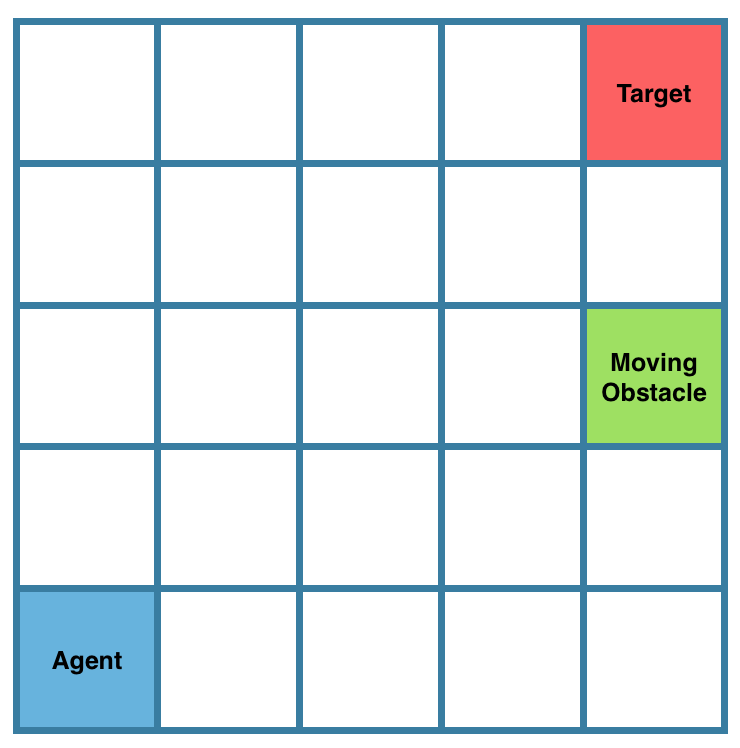
\includegraphics[width=0.5\columnwidth]{images/gridworld.png}
  \caption{Moving obstacle gridworld 	\label{fig:gridworld}}
\end{figure}
\begin{table}[]
\centering

\label{tab:results}
\begin{tabular}{|l|l|l|l|}
\hline
           & $\lambda_e(\Phi_{a}-\Phi_{e)}$& $\lambda_t(\Phi_{a}-\Phi_{t)}$ & $|\pi_a - \pi_t|$ (\%) \\ \hline
Original   & -6.125(2.06)        & 2.41(1.82)         & 15                    \\ \hline
Our Method & 0(0.2)              & 0.02(0.167)        & 10                    \\ \hline
\end{tabular}
\caption{Results on test set after 20 runs of random initial conditions. $\lambda_e$ represent reward weights, $\pi$ represents policy and $\Phi$ represents feature expectations. The subscripts $a,e,t$ represent the apprentice, expert and taboo agents respectively. \jm{This table needs to be cleaned up. Try to keep the same number of significant figures in all entries.}}
\end{table}
It should be apparent from the results, \sw{These results show...} that using the additional data of avoidable behaviour \sw{don't use new words for concepts you've already introducted} allows the apprentice to 
come closer to the actual desired behaviour, which is that of the expert. Furthermore, in the third row of Table .. we can see that
even if the apprentice is trained only on the taboo agent, his policy and performance still come closer to the expert \sw{than what?}. This is further
evidence that learning to imitate and learning to avoid behaviours are related concepts and should be used interchangeable depending on the application. \sw{I don't understand this claim.}

\begin{figure}[t]
  \centering
  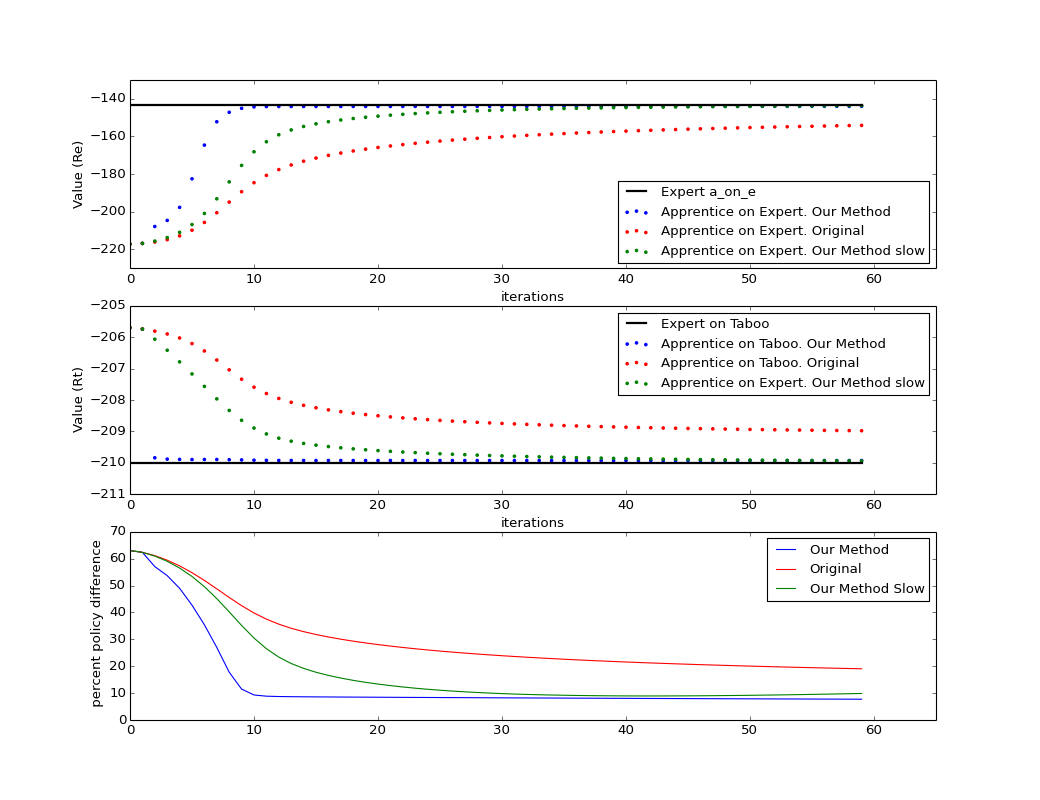
\includegraphics[width=0.9\columnwidth]{images/testgraph}
  \caption{A typical run for moving obstacle gridworld. Our method (blue) will quickly outperform the original algorithm. Achieving value that is closer to that of the expert, and reducing the difference with the desired policy\label{fig:results}}
\end{figure}

\subsection{Real Social Navigation Data.}




\section{Related Work}

\sw{Given that space will be tight, this should just be folded into the rest of the paper: mention each ref when it is relevent, primarily in background, but also in method and experiments.}

Inverse Reinforcement Learning was introduced by \cite{ng2000algorithms} and \cite{abbeel2004apprenticeship}. The first probabilistic interpretation of the framework was introduced by Ramachandran and Amir 2007 and extended to Maximum Entropy IRL by Ziebart et al 2009. 	Learning from failure is an area that has found most attention in the Robotics community and specifically imitation learning. \cite{choi2015} introduces leveraged non stationary Gaussian processes, that fit good data points while trying to avoid bad ones. The method was also applied to robotic navigation, but not in terms of IRL. \cite{grollman2012robot} Use past failures of the robot to initialise robot policies, and conclude that there is indeed information in failed trajectories that should not be discarded. IRL has been previously applied to social robot navigation, notable works are those of \cite{henry2010learning} and \cite{vasquez2014inverse}, that use pedestrian simulators to extract the underlying reward function of a human controller. To our knowledge our work is the first to implement Learning from Failure in Inverse Reinforcement Learning and assess its performance using real social navigation data.

\section{Conclusions and Future Work}

\sw{This can be modeled on the new abstract once it's written.  We do need some future work ideas.} \jm{Perhaps we can mention further robot tests and validation of these results as future work. There was also this idea on the table of coupling this learning from failure approach with other IRL / LfD algorithms}

In this paper we have introduced a new framework for Inverse Reinforcement Learning that allows an agent to not only imitate certain behaviours but to also avoid others. The benefits this approach is that it allows otherwise useless data to be used and further enables a designer to inject prior information in the learning, by specifying, through simulated data, what behaviours should be avoided. We have derived a theoretically sound method by directly modifying the derivation of the Maximum Entropy and carrying that through to MaxEnt IRL, providing solutions to the computational obstacles that arise. We have further performed exhaustive experiments in a toy domain, that clearly demonstrate that our method can generalise much better that the baseline IRL algorithm. Finally we have performed learning on real data, again showing that our method is superior to the baseline.  

\bibliographystyle{aaai}
\bibliography{references}
	
\end{document}
